\documentclass{beamer}
% This is the file main.tex
%\usetheme{default}
\usetheme{CambridgeUS}
%\usecolortheme{seahorse}
\usecolortheme{rose}
\usefonttheme[onlylarge]{structuresmallcapsserif}
\usefonttheme[onlysmall]{structurebold}
%\setbeamerfont{title}{shape=\itshape,family=\rmfamily}
%\setbeamercolor{title}{fg=red!80!black}
%\setbeamercolor{title}{fg=red!80!black,bg=red!20!white}

% Utilizamos el paquete para usar español
\usepackage[spanish]{babel}
% Utilizamos un paquete para gestionar los acentos
% y las e ¿es
\usepackage[utf8]{inputenc}
% amsmath y amssymb de la American Mathematical 
% Society (fórmulas matemáticas)
\usepackage{amsmath}
\usefonttheme[onlymath]{serif}
%Para que reconozca el entorno verbatim
\usepackage{fancyvrb}
%Definimos nuestra ruta para las imagenes
%Absoluto
%\graphicspath{ {/home/user/images/} }
%Relativo (recomendado) -> según
%https://es.sharelatex.com/learn/Inserting_Images#La_ruta_a_la_carpeta_de_im.C3.A1genes
\graphicspath{ {media/} }


\title[Curso RedPitaya]{Requerimientos HW y SW}
\subtitle{Universidad Nacional de Rio Negro \\ S. C. de Bariloche}
\author[\texttt{@horacio\_arnaldi}]{Horacio Arnaldi \\ \texttt{{\href{mailto:arnaldi@cab.cnea.gov.ar}{arnaldi@cab.cnea.gov.ar}}}}
\institute[LabDPR - CAB - IB]{Laboratorio Detección de Partículas y Radiación \\ Centro Atómico Bariloche - Instituto Balseiro}
%\date{\today}
\date{}

\begin{document}

\begin{frame}
\hspace*{1.2cm}
\includegraphics[height=0.18\textheight]{cnea_logo} \hspace*{2cm}
\includegraphics[height=0.18\textheight]{balseiro_logo} \hspace*{2cm}
\includegraphics[height=0.18\textheight]{LabDPR_logo} %\hspace*{1cm}
%\includegraphics[height=0.18\textheight,width=0.15\textwidth]{logos/lagologo}

\titlepage

\end{frame}

\begin{frame}
\frametitle{Contenido}
\setcounter{tocdepth}{1} %para incluir solo las secciones en el TOC
\tableofcontents
%  \tableofcontents[pausesections]
\end{frame}

%------------------------------------------------------------------------------
\section{Introducción}
%------------------------------------------------------------------------------

\begin{frame}
\begin{center}
\Huge{\color{blue}{Introducción}}
\end{center}
\end{frame}

\begin{frame}
\frametitle{Introducción}
\only<1>{\fbox{\includegraphics[width=0.4\textwidth]{rp_tipos}}}
\only<2>{\fbox{\includegraphics[width=0.5\textwidth]{signal_lab}}}
\end{frame}

%FIXME: ver si incluir el principio del Knoll donde habla de fuentes de radiación, como para entrar en contexto de qué es lo que queremos medir
\begin{frame}
\begin{block}{Introducción}
\begin{itemize}
\item Describiremos y definiremos algunas catacterísticas generales, comunes a los
detectores, las señales y el ruido asociado a ellos
\item Principio fundamental: \alert{La transferencia de parte o toda la energía
de radiación a la masa del detector donde es convertida a otra forma más
accesible para la percepción humana}
\item Las partículas cargadas transfieren su energía a la materia a través de
colisiones directas con los electrones atómicos, induciendo
{\color{blue}excitación} o {\color{blue}ionización} en los átomos
\item La radiación neutra, por otro lado, primero debe producir algún tipo de
reacción en el detector producciendo partículas cargadas, las cuales a su vez
ionizan y excitan los átomos del detector
\end{itemize}
\end{block}
\end{frame} 

\begin{frame}
\begin{block}{Introducción (cont.)}
\begin{itemize}
\item La forma en la que la energía convertida aparece {\color{blue}depende del detector y de
su diseño}
\item Los detectores modernos de hoy en día son esencialmente
eléctricos/electrónicos
\item En algún punto la información proveniente del detector es
tranformada a pulsos eléctricos, los cuales pueden tratarse con técnicas
electrónicas
\item Cuando hablamos de ``detectores'' estamos, entonces, teniendo en cuenta su
electrónica asociada también
\end{itemize}
\end{block}
\end{frame} 

\begin{frame}
\frametitle{Elección del detector}
\begin{alertblock}{Factores de decisión}
\begin{itemize}
\item La región de longitudes de onda de la radiación 
\item La intensidad de la radiación
\item La respuesta temporal requerida para resolver eventos de alta
velocidad
\item La superficie de detector requerida
\item El ambiente en el cual el detector será usado
\item El costo
\item La electrónica asociada al detector
\end{itemize}
\end{alertblock}
\end{frame} 

%esta parte sigue los lineamientos de Spieler Introducción
%------------------------------------------------------------------------------
\subsection{¿Por qué?}
%------------------------------------------------------------------------------

\begin{frame}
\frametitle{¿Por qué?}
{
\setbeamercolor{block body}{bg=red!20, fg=blue}
\begin{block}{}
La radiación es el único {\color{red}observable} en procesos que ocurren en una escala que es
demasiado breve o demasiado pequeña para ser observada directamente. También es
el único acceso a procesos que están muy lejos.
\end{block}
}
\begin{block}{}
Originalmente desarrollado para la física de partículas atómica, nuclear y
elemental, los detectores de radiación ahora se aplican en muchas áreas diversas
de la ciencia, la ingeniería y la vida cotidiana.
\end{block}
{
\setbeamercolor{block body}{bg=green!20}
\begin{block}{}
El progreso en la ciencia no sólo es impulsado por la interacción de la teoría y
el experimento, sino también por los avances en la {\color{blue}instrumentación}
\end{block}
}
\end{frame}

\begin{frame}
\frametitle{Tipos de radiación}
\begin{alertblock}{}
\begin{itemize}
\item[a] Partículas cargadas 
\begin{itemize}
\item {\color{blue}electrones, protones, núcleos atómicos, partículas
elementales} 
\end{itemize}
\item[b] Partículas neutras 
				\begin{itemize}
\item {\color{blue}neutrones, partículas elementales, gravitones
elementales} 
				\end{itemize}
\item[c] Fotones 
				\begin{itemize}
\item {\color{blue}ondas milimétricas, rayos gamma, rayos X, luz
elementales} 
				\end{itemize}
				\end{itemize}
				\end{alertblock}
				\end{frame}

				\begin{frame}
\frametitle{La mayoría de los detectores modernos convierten la
energía absorvida en una señal eléctrica}
\begin{alertblock}{La sensibilidad de la detección depende de:}
\begin{itemize}
\item fluctuaciones en el detector
\item fluctuaciones en la electrónica
\end{itemize}
\end{alertblock}
\begin{exampleblock}{Para maximizar la sensibilidad en la detección se
deben considerar:}
\begin{itemize}
\item la formación de la señal en el detector
\item el acoplamiento del detector a la electrónica
\item las fluctuaciones en la electrónica
\end{itemize}
\end{exampleblock}
\end{frame}

\begin{frame}
\frametitle{\small{El desarrollo de sistemas detectores es una mezcla interdisciplinaria de física y electrónica}}
{
\setbeamercolor{block body}{bg=blue!20}
\small{Por ejemplo, la comprensión de un detector moderno de tracking
(seguimiento) en física de altas energías o de un sistema de imágenes médicas
requiere conocimientos de:}
\begin{itemize}
\item física de estado sólido
\item física de dispositivos semiconductores
\item tecnología de fabricación de semiconductores
\item técnicas para electrónica de bajo ruido
\item microelectrónica analógica y digital
\item transmisión de datos a altas velocidades
\item sistemas de adquisición de datos basados en computadoras
\end{itemize}
}
\begin{exampleblock}{}
\small{¡Es decir que es una gran forma de aprender sobre la interrelación de la
\alert{física} con la \alert{tecnología}!}
\end{exampleblock}
\end{frame}

%------------------------------------------------------------------------------
\subsection{Ejemplos}
%------------------------------------------------------------------------------

%------------------------------------------------------------------------------
\subsection{El problema}
%------------------------------------------------------------------------------

\begin{frame}
\frametitle{El problema}
\begin{alertblock}{}
\begin{itemize}[<+->]
\item La radiación afecta a un sensor y genera una señal eléctrica

\item El nivel de señal es bajo y debe amplificarse para permitir la digitalización y
el almacenamiento

\item Tanto el sensor como los amplificadores introducen fluctuaciones de señal/ruido
\begin{enumerate}
\item Fluctuaciones en la señal introducida por el sensor
\item Ruido de la electrónica superpuesta a la señal
\end{enumerate}

\item El límite de detección y la precisión de la medición están
determinados por la relación señal/ruido (SNR)
\end{itemize}
\end{alertblock}

\only<7>{\begin{alertblock}{¿Cómo optimizar la relación señal/ruido?}
\begin{enumerate}
\item Aumentar la señal y reducir el ruido
\item Para un sensor y una señal dada: {\color{blue}reducir el ruido
electrónico}
\end{enumerate}
\end{alertblock}}
\end{frame}

\begin{frame}
\frametitle{Ejemplo}
\begin{block}{}
\includegraphics[height=0.35\textheight,width=\textwidth]{d1/espectro_pulso_unipolar} \\
\includegraphics[height=0.35\textheight,width=\textwidth]{d1/espectro_pulso_bipolar} 
\end{block}
\end{frame} 

\begin{frame}
\frametitle{\small{El espectro de ruido generalmente es distinto al de la
señal}}
\begin{columns}
\begin{column}{0.5\textwidth}
\begin{block}{\small{Espectro de ruido típico}}
\includegraphics[height=0.4\textheight,width=\textwidth]{d1/espectro_ruido_tipo}
\end{block}
\end{column}
\begin{column}{0.48\textwidth}
\begin{alertblock}{}
Adaptar la respuesta en frecuencia del sistema de medición para optimizar la
relación señal/ruido
\end{alertblock}
\end{column}
\end{columns}
\begin{block}{}
La respuesta en frecuencia del sistema de medición \alert{afecta a los dos}: señal y
ruido
\end{block}
\end{frame} 

\begin{frame}
\frametitle{Pasos para el análisis de un sistema de procesamiento de pulsos}
\begin{exampleblock}{}
\begin{itemize}
\item Determinar la magnitud de la señal y su dependencia temporal 
\begin{itemize}
\item Estos dependerán de cómo está acoplado el sistema de medición al sensor
$\rightarrow$ \alert{modelo} para el detector
\end{itemize}
\item Determinar el origen y la magnitud de las fluctuaciones 
\begin{itemize}
\item fluctuaciones de la señal
\item ruido aleatorio
\item interferencia externa
\end{itemize}
\item Diseñar el sistema de filtrado (optimizar SNR)
\item Determinar el sistema de lectura y digitalización de datos a utilizar
\end{itemize}
\end{exampleblock}
\end{frame} 

\begin{frame}
\frametitle{Un sistema detector grande puede consistir en varios
subsistemas especialmente diseñados para realizar funciones específicas}
\begin{exampleblock}{Ejemplos}
\begin{itemize}
\item Sensado de posición (tracking)
\item Medición de energía (espectroscopia, calorímetros)
\item Medición de tiempos
\item Identificación de partículas
\end{itemize}
\end{exampleblock}
\end{frame} 

\subsection{Funciones}

\begin{frame}
\frametitle{Características generales de los detectores}
\framesubtitle{{\color{blue}Funciones}}
\begin{exampleblock}{}
Aunque esos subsistemas sean distintos y usen tecnologías
distintas, realizan básicamente las mismas funciones:
\end{exampleblock}
\begin{block}{1-La radiación deposita su energía en un medio detector}
\begin{itemize}
\item[-] El medio puede ser {\color[rgb]{0.82,0.1,0.26}gas, líquido o sólido}

\item[-] En un detector de seguimiento se desea detectar la presencia de una partícula
sin afectar su trayectoria, por lo que \alert{el medio se elegirá para minimizar la
pérdida de energía y la dispersión de partículas}

\item[-]En cambio, si se desea medir la energía total (espectrometría o calorimetría),
el medio se elegirá para optimizar la pérdida de energía (alta densidad, Z alta)
\end{itemize}
\end{block}
\end{frame} 

\begin{frame}
\frametitle{Características generales de los detectores}
\framesubtitle{{\color{blue}Funciones}}
\begin{block}{2-La energía se convierte en una señal eléctrica, directa o
indirectamente. Cada partícula detectada aparecerá como un pulso de carga
eléctrica}
\begin{itemize}
\item[-] {\color[rgb]{0.5,0,0.13}Conversión directa:}

La radiación incidente ioniza átomos/moléculas en el medio absorbente,
creando cargas móviles que se detectan (cámara de ionización)

\item[-] {\color[rgb]{0.5,0,0.13}Conversión indirecta:}

La radiación incidente excita estados atómicos/moleculares que se descomponen
por emisión de luz, que en una segunda etapa se convierte en carga (detectores
de centelleo)
\end{itemize}
\end{block}
\end{frame} 

\begin{frame}
\frametitle{Características generales de los detectores}
\framesubtitle{{\color{blue}Funciones}}
\small{{\color{blue}La carga de la señal primaria es proporcional a la energía
absorbida}}

\small{Algunos valores típicos de energía requeridos para formar una señal de carga
correspondiente a 1 electrón:}
\begin{center}
gases\hspace{2cm}   \alert{$30\,eV$}

semiconductores\hspace{1cm}   \alert{1 a $10\,eV$ }

centelladores\hspace{1.9cm}    \alert{20 a $500\,eV$}
\end{center}
\begin{alertblock}{\small{En ninguno de estos esquemas la carga de la señal está
disponible instantáneamente}}
\small{En un detector de centelleo la duración del pulso se determina por el tiempo de
decaimiento de las transiciones ópticas

En una cámara de ionización las cargas deben moverse a los electrodos para
obtener la señal completa}

\begin{center}
duración típica de los pulsos\hspace{.5cm} \alert{$1\,ns - 10\,\mu s$}  
\end{center}
\end{alertblock}
\end{frame} 

\begin{frame}
\frametitle{Características generales de los detectores}
\framesubtitle{{\color{blue}Funciones}}
\begin{block}{3-La señal eléctrica es amplificada}
\begin{enumerate}
\item {\color[rgb]{0.5,0,0.13}Circuitería electrónica}
\item {\color[rgb]{0.5,0,0.13}Ganancia por medio de multiplicación secundaria}

La carga primaria se acelera con suficiente energía para liberar los portadores
de carga adicionales a través de ionización por impacto

Ejemplos:

\alert{Cámaras proporcionales}

\alert{Fotodiodos de avalancha}

\alert{Fotomultiplicador}
\end{enumerate}
\end{block}
\begin{alertblock}{}
Ambas técnicas pueden introducir fluctuaciones significativas (ruido)
\end{alertblock}
\end{frame} 

\begin{frame}
\frametitle{Características generales de los detectores}
\framesubtitle{{\color{blue}Funciones}}
\begin{block}{Idealmente, una etapa de ganancia sólo debería aumentar la magnitud del
pulso, sin afectar su dependencia temporal}

Este comportamiento ideal nunca se realiza en la práctica, ya que
\alert{requeriría amplificadores con un ancho de banda infinito}

\vspace*{10mm}

{\color[rgb]{0,0.26,0.15}Esto no es una limitación severa, ya que en muchas
aplicaciones resulta aceptable e incluso deseable cambiar la forma del pulso}
\end{block}
\end{frame} 

\begin{frame}
\frametitle{Características generales de los detectores}
\framesubtitle{{\color{blue}Funciones}}
\begin{block}{4-Conformación del pulso (pulse shaping)}
\begin{alertblock}{}
No siempre necesario, pero siempre presente de alguna forma
\end{alertblock}
La respuesta temporal del sistema se adapta para \alert{optimizar} la medición
de la {\color{blue}magnitud o el tiempo} de la señal y {\color{blue}la velocidad} de detección
de la señal
\end{block}

\begin{exampleblock}{}
{\color[rgb]{0.5,0,0.13}La salida de la cadena de señal es un pulso (corriente o
voltaje) cuya área es proporcional a la carga de la señal original, es decir, la
energía depositada en el detector}
\end{exampleblock}
\end{frame} 

\begin{frame}
\frametitle{Características generales de los detectores}
\framesubtitle{{\color{blue}Funciones}}
\begin{block}{}
Típicamente, el conformador de pulsos transforma un pulso de
corriente \alert{estrecho} del detector en un pulso más \alert{amplio} (para
reducir el ruido electrónico), con un máximo gradualmente redondeado en un
tiempo $T_p$ (para facilitar la medición de la amplitud)
\end{block}

%\begin{exampleblock}{}\centering
\includegraphics[height=0.45\textheight,width=0.9\textwidth]{d1/det_pulse_and_shaper_out}
%\end{exampleblock}{}
\end{frame} 

\begin{frame}
\frametitle{Características generales de los detectores}
\framesubtitle{{\color{blue}Funciones}}
\begin{block}{}
Si la forma del pulso no cambia con el nivel de señal, la amplitud de pico es
también una medida de la energía, por lo que a menudo se habla de \alert{medidas de
altura de pulso o análisis de altura de pulso}. 

{\color[rgb]{0.5,0,0.13}El espectro de altura de pulso es el espectro de
energía}
\end{block}

%\begin{exampleblock}{}
\begin{center}
\includegraphics[height=0.45\textheight,width=0.6\textwidth]{d1/pulse_height_spectrum}
\end{center}
%\end{exampleblock}{}
\end{frame} 

\begin{frame}
\frametitle{Características generales de los detectores}
\framesubtitle{{\color{blue}Funciones}}
\begin{block}{5-Digitalización de:}
\begin{itemize}
\item[1-] {\color[rgb]{0.5,0,0.13}\small{La magnitud de la señal (conversor
A/D)}}

\item[2-] {\color[rgb]{0.5,0,0.13}\small{Diferencia de tiempo entre una señal de
referencia y la señal detectada (time-to-digital converter, TDC)}}

\small{La señal de referencia puede derivarse de otro detector (como en time-of-flight
PET, TOF-PET) o de un reloj de sistema común}

%Las implementaciones de circuitos incluyen esquemas que cuentan ``ticks de
%reloj'' en circuitería completamente digital o combinan conversión de tiempo a
%amplitud y de amplitud a digital en arreglos mixtos analógico-digitales}
\end{itemize}
\end{block}

\begin{exampleblock}{}
{\color[rgb]{0.5,0,0.13}\small{En sistemas de detección complejos, las salidas
digitalizadas individuales pueden requerir circuitos bastante complejos para
combinar la señal asociada con un evento específico y ``empaquetarlos'' para una
transferencia eficiente}}
\end{exampleblock}
\end{frame} 

\subsection{Características generales de los detectores}
%Esta parte la saco del libro de W. Leo, ch5

\begin{frame}
\frametitle{Características generales de los detectores}
\framesubtitle{{\color{blue}Eficiencia}}
\begin{exampleblock}{}
Generalmente se hace referencia a dos tipos de eficiencia cuando se habla de
detectores de radiación:
\begin{itemize}
\item {\color{blue}Eficiencia total o absoluta}: depende no solo de las propiedades del
detector, sino también de los detalles de la geometría del proceso de conteo
(p.ej. de la distancia entre la fuente y el detector)
\item {\color{blue}Eficiencia intrínseca de detección}: depende del material del
detector, de la energía de la radiación y del espesor del detector en la
dirección de la radiación incidente 
\end{itemize}
\end{exampleblock}
\end{frame} 

\begin{frame}
\frametitle{Características generales de los detectores}
\framesubtitle{{\color{blue}Eficiencia}}
\begin{block}{Eficiencia absoluta} 
$$\textit{E}_{tot} = \frac{\text{eventos registrados}}{\text{eventos emitidos por
la fuente}}$$
\end{block}
\begin{block}{Eficiencia intrínseca} 
$$\textit{E}_{int} = \frac{\text{eventos registrados}}{\text{eventos que inciden
en el detector}}$$
\end{block}
\begin{block}{Las dos eficiencias están relacionadas} 
$$\textit{E}_{int} = \textit{E}_{abs} \frac{4 \pi}{\Omega}$$
$\Omega$ es el ángulo sólido del detector visto desde la posición de la fuente 
\end{block}
\end{frame} 

\begin{frame}
\frametitle{Características generales de los detectores}
\framesubtitle{{\color{blue}Sensibilidad}}
\begin{exampleblock}{}
Capacidad de producir una señal usable para un tipo de radiación y energía
determinados 
\end{exampleblock}
\begin{alertblock}{}
\begin{itemize}
\item Definida para un tipo de radiación y para un cierto rango de
energías 
\item Fuera de ese rango decrece la \alert{eficiencia}
\end{itemize}
\end{alertblock}
\begin{block}{Factores que influyen}
\begin{itemize}
\item Sección transversal para las reacciones de ionización en el
detector
\item La masa del detector 
\item	El ruido inherente del detector
\item	El material de proteccción en los alrededores del volumen sensible
del detector 
\end{itemize}
\end{block}
\end{frame} 

\begin{frame}
\frametitle{Respuesta del detector}
\begin{exampleblock}{}
\begin{itemize}
\item Hace referencia a la capacidad del detector de proveer información no sólo
de la presencia de radiación, sino también de la energía de esa radiación 
\item En general, la señal de salida de los detectores eléctricos es en la forma
de un pulso de corriente 
\item La cantidad de ionización se refleja en la carga eléctrica contenida en la
señal
\end{itemize}
\end{exampleblock}
\begin{alertblock}{}
\begin{itemize}
\item Definida para un tipo de radiación y para un cierto rango de
energías 
\item Fuera de ese rango decrece la eficiencia
\end{itemize}
\end{alertblock}
\end{frame} 

\subsubsection{Resolución en energía. El factor de Fano}

\begin{frame}
\frametitle{Resolución}
\begin{alertblock}{}
\begin{itemize}
\item La resolución se da usualmente en términos del \alert{ancho a media altura del
máximo (\textit{full width at half maximum (FWHM)}}) 
\end{itemize}
\end{alertblock}
\begin{center}
\includegraphics[width=0.7\textwidth]{d1/det_resolution_definition}
\end{center}
\end{frame} 

\begin{frame}
\frametitle{Resolución}
\begin{alertblock}{}
\begin{itemize}[<+->]
\item Rangos menores de energía que este intervalo se consideran irresolubles 
\item Para pulsos cuya forma es Gaussiana con desviación estándar $\sigma$, $FWHM = 2.35\,\sigma$
$$R = \frac{\Delta E}{E}$$
\end{itemize}
\end{alertblock}
\begin{center}
\only<1>{\includegraphics[width=0.45\textwidth]{d1/resolucion_dos_picos}}
\only<2>{\includegraphics[width=0.45\textwidth]{d1/det_resolution_definition}}
\only<3>{\includegraphics[width=0.45\textwidth]{d1/energy_resolution_det}}
\end{center}
\end{frame} 

\subsubsection{La función de respuesta}

\subsubsection{Tiempo de respuesta}

\begin{frame}
\frametitle{Tiempo de respuesta}
\begin{exampleblock}{}
\begin{itemize}
\item Hace referencia al tiempo que le toma al detector formar la señal después de que la radiación ha arribado
\end{itemize}
\end{exampleblock}
\begin{alertblock}{}
\begin{itemize}
\item La duración de la señal también es importante: \alert{durante 
este período un segundo evento no puede ser aceptado, ya 
sea porque el detector es insensible o porque la segunda 
señal se apila (pile-up) con la primera}
\item Estos factores contribuyen al \alert{tiempo muerto} del detector 
y limita la tasa de conteo a la cual puede operarse el detector
\end{itemize}
\end{alertblock}
\end{frame} 

\subsubsection{Eficiencia del detector}

\subsubsection{Tiempo muerto}

%------------------------------------------------------------------------------
\section{Ruido}
%------------------------------------------------------------------------------
%esta parte está en pág.565 de Building Scienti...

\begin{frame}
\frametitle{Ruido}
\framesubtitle{Ruido en el proceso de detección}
\begin{itemize}
\item El ruido es una señal indeseada
\item Está presente en algún grado en todos los sistemas
\item Resulta de interés cuando oscurece (tapa) una señal deseada
\end{itemize}
\begin{center}
\includegraphics[width=0.55\textwidth]{d1/environmental_noise_spectrum}
\end{center}
\end{frame} 

\begin{frame}
\frametitle{Ruido}
\framesubtitle{Ruido en el proceso de detección}
\begin{columns}
\begin{column}{0.5\textwidth}
\begin{block}{Ruido determinístico}
\begin{itemize}
\item Simples componentes de frecuencia discreta (armónicos de línea, 50 o 60 Hz)
\item Interferencia de radiofrecuencia (RFI) (p.ej. pulsos estrechos de alta
energía debido a fuentes conmutadas)
\item Láseres pulsados
\item Transmisores de radar
\end{itemize}
\end{block}
\end{column}
\begin{column}{0.5\textwidth}
\begin{center}
\includegraphics[width=\textwidth]{d1/environmental_noise_spectrum}
\end{center}
\end{column}
\end{columns}
\end{frame} 

\begin{frame}
\frametitle{Ruido}
\framesubtitle{Ruido en el proceso de detección}
\begin{columns}
\begin{column}{0.5\textwidth}
\begin{block}{Ruido aleatorio (estocástico)}
\begin{itemize}
\item Ruido blanco, donde la densidad espectral de potencia es
independiente de la frecuencia
\begin{itemize}
\item Ruido Johnson
\item Ruido de disparo 
\end{itemize}
\item Ruido flicker o $1/f$, donde la densidad espectral de potencia disminuye a
medida que aumenta la frecuencia
\end{itemize}
\end{block}
\end{column}
\begin{column}{0.5\textwidth}
\begin{center}
\includegraphics[width=\textwidth]{d1/environmental_noise_spectrum}
\end{center}
\end{column}
\end{columns}
\end{frame} 

\begin{frame}
\frametitle{Ruido}
\framesubtitle{Ruido en el proceso de detección}
\begin{block}{Densidad espectral de potencia}
Se mide en unidades de $<\!v_N\!>^2/\text{Hz}$ o $<\!i_N\!>^2/\text{Hz}$

Si se tiene una tensión RMS de $v$ voltios y un rango de frecuencias $\Delta f$
Hz, la densidad espectral de potencia, $S$, viene dada por
{\color{blue}$$S = \frac{v^2}{\Delta f} = \left(\frac{v}{\sqrt{(\Delta
f)}}\right)^2$$}

$v/\sqrt{(\Delta f)} \rightarrow$ \textit{densidad espectral de tensión}
[$\text{voltios RMS}/\sqrt{\text{Hz}}$]
\end{block}
\end{frame} 

\begin{frame}
\frametitle{Ruido}
\framesubtitle{Ruido en el proceso de detección}
\begin{itemize}
\item El ruido es la \alert{tensión o corriente fluctuante al azar} producida por el
detector y su electrónica asociada
\item El ruido fluctúa positivamente y negativamente alrededor de cero en una
escala de tiempo que está determinada por la respuesta en frecuencia del sistema
que lo genera
\item Si el ruido se caracteriza por una corriente $i_N$, la corriente de ruido
media es $<\!i_N\!> = 0$
\item El ruido debe caracterizarse por su valor cuadrático medio, promediado
durante un tiempo suficientemente largo \alert{$<\!i_N\!>^2$}
\item Esto se denomina a menudo {\color{blue}potencia de ruido}, aunque estrictamente
hablando, la potencia de ruido es \alert{$<\!i_N\!>^2 R$}, donde $R$ es una
{\color{blue}resistencia efectiva} a través de la cual fluye la corriente de ruido
\end{itemize}
\end{frame} 

%\begin{frame}
%\frametitle{Ruido electrónico}
%\begin{exampleblock}{Ruido en el proceso de detección}
%\begin{itemize}
%\item Ruido de disparo (shot noise, photon noise o quantum noise)
%\item Ruido Johnson (thermal noise o Nyquist noise)
%\item Ruido $1/f$ (flicker noise, current noise o excess noise)
%\end{itemize}
%\end{exampleblock}
%\end{frame} 

\begin{frame}
\frametitle{Ruido electrónico y resolución}
\framesubtitle{¿Por qué? \\ Resolución: habilidad de distinguir niveles de señal}
{\color{blue}Reconocimiento de estructuras en espectros de amplitud}
%\begin{exampleblock}{Reconocimiento de estructuras en espectros de amplitud}
\begin{center}
\only<1>{\includegraphics[width=0.8\textwidth]{d1/NaI_v_Ge_PIN_resolution}}
\only<2>{\includegraphics[height=0.65\textheight,width=0.5\textwidth]{d1/NaI_v_Ge_PIN_resolution2} \\
\tiny{(J.Cl. Philippot, IEEE Trans. Nucl. Sci. NS-17/3 (1970) 446)}}
\end{center}
%\end{exampleblock}
\end{frame} 

\begin{frame}
\frametitle{Ruido electrónico y resolución}
\framesubtitle{¿Por qué?}
{\color{blue}Mejora en la sensibilidad} \\
\small{La relación entre la señal y el fondo mejora con una mejor resolución}
%\begin{exampleblock}{Mejora en la sensibilidad}
\begin{center}
\includegraphics[height=0.68\textheight,width=0.5\textwidth]{d1/improved_sensitivity} \\
\tiny{(G.A. Armantrout et al., IEEE Trans. Nucl. Sci. NS-19/1 (1972) 107)}
\end{center}
%\end{exampleblock}
\end{frame} 

\begin{frame}
\frametitle{Ruido electrónico y resolución}
\framesubtitle{¿Qué determina la resolución?}
{\color{blue}Caso 1: Variancia de la señal $\gg$ Variancia de la linea de base} 
%\begin{exampleblock}{Mejora en la sensibilidad}
\begin{center}
\includegraphics[height=0.5\textheight,width=\textwidth]{d1/signal_mayor_baseline} 
\end{center}
%\end{exampleblock}
\end{frame} 

\begin{frame}
\frametitle{Ruido electrónico y resolución}
\framesubtitle{¿Qué determina la resolución?}
{\color{blue}Caso 1: Variancia de la señal $\gg$ Variancia de la linea de base} 
\begin{alertblock}{}
Ruido electrónico (línea de base) sin (o escasa) importancia
\end{alertblock}
\begin{block}{Ejemplo: \footnotesize{rayos gamma de $1\,MeV$ absorvidos por un cristal de $NaI(Tl)$}}
Nº de pe $\rightarrow N_{pe} \approx
8\cdot10^4\,[MeV^{-1}]\,\text{x}\,E_{\gamma}\,\text{x}\,QE \approx 2.4\cdot10^4$

\vspace{1mm}
Variancia típica $\rightarrow \sigma_{pe} = N_{pe}^{1/2} \approx 160$ y
$\sigma_{pe}/N_{pe} \approx 5 - 8\,\%$ 

\vspace{1mm}
Señal en el ánodo del PMT (asumiendo una ganacia $G_{PMT} = 10^4$) $\rightarrow$  
\begin{center}
$Q_{sig} = G_{PMT}N_{pe} \approx 2.4\cdot10^8\,e^-$  

\vspace{1mm}
y $\sigma_{sig} = G_{PMT}\sigma_{pe}
\approx 1.2\cdot10^7\,e^-$ 
\end{center}

\alert{mientras que el ruido electrónico es fácilmente $< 10^4\, e^-$}
\end{block}
\end{frame} 

\begin{frame}
\frametitle{Ruido electrónico y resolución}
\framesubtitle{¿Qué determina la resolución?}
{\color{blue}Caso 2: Variancia de la señal $\ll$ Variancia de la linea de base} 
%\begin{exampleblock}{Mejora en la sensibilidad}
\begin{center}
\includegraphics[height=0.5\textheight,width=\textwidth]{d1/baseline_mayor_signal} 
\end{center}
%\end{exampleblock}
\end{frame} 

\begin{frame}
\frametitle{Ruido electrónico y resolución}
\framesubtitle{¿Qué determina la resolución?}
{\color{blue}Caso 2: Variancia de la señal $\ll$ Variancia de la linea de base} 
\begin{alertblock}{}
Ruido electrónico (línea de base) crítico para la resolución
\end{alertblock}
\begin{block}{Ejemplo: \footnotesize{en detectores de $Si$}}
Nº de pares electrón-hueco $\rightarrow$
\begin{center}
$N_{ep} = E/\varepsilon_i \quad (E = \text{energía absorbida,}\, \varepsilon_i = 3.6\,\text{eV} (\text{energía de ionización}))$ 
\end{center}

Variancia típica $\rightarrow$ 
\begin{center}
$\sigma_{ep} = \sqrt{F\cdot N_{ep}} \quad (\text{donde} \,\, F = \text{Factor de Fano} \approx 0.1)$
\end{center}

Para fotones de $50\,\text{keV} \rightarrow$
$\sigma_{ep} \approx 40\,e^- \implies
\sigma_{ep}/N_{ep} = 7.5\cdot10^{-4}$

\vspace{2mm}
\alert{los niveles de ruido obtenibles van de 10 a $1000\,e^-$}
\end{block}
\end{frame} 

\begin{frame}
\frametitle{Ruido electrónico y resolución}
\framesubtitle{¿Qué determina la resolución?}
\begin{block}{}
Las fluctuaciones de la linea de base pueden tener distintos orígenes:

captación de interferencias externas ...

artefactos debido a la electrónica imperfecta ...

etc.

\alert{pero el límite fundamental (práctico) es el {\color{blue}ruido
electrónico}}
\end{block}
\end{frame} 

\begin{frame}
\frametitle{Mecanismos básicos de ruido}
\begin{block}{}
Si consideramos $n$ portadores de carga $e$ moviéndose
con una velocidad $v$ a través de una muestra de longitud
$l$. La corriente inducida $i$ en los extremos de la muestra es
$$i = \frac{nev}{l}$$
La fluctuación de esa corriente viene dada por el diferencial total

$$\langle di \rangle^2 = \left(\frac{ne}{l}\langle dv \rangle \right)^2 +
\left(\frac{ev}{l}\langle dn \rangle \right)^2 $$

donde los dos términos \alert{se suman cuadráticamente debido a que corresponden a ruido
no correlacionado estadísticamente}
\end{block}
\end{frame} 

\begin{frame}
\frametitle{Mecanismos básicos de ruido}
%\begin{block}{}
{\color{blue}Dos mecanismos contribuyen al ruido}
\begin{itemize}
\item fluctuaciones de velocidad $\rightarrow$ {\color[rgb]{0.8,0.33,0}ruido térmico}
\item fluctuaciones en el número de portadores $\rightarrow$
{\color[rgb]{0.43,0.21,0.1}ruido de disparo / ruido
$1/f$}
\end{itemize}
%\end{block}
%\begin{block}{}
El ruido térmico y el ruido de disparo son ambas fuentes de ruido ``blanco'', es
decir, la potencia por unidad de ancho de banda es constante (\alert{densidad
espectral}):

$$\frac{dP_{noise}}{df} = const. \quad o
\quad \frac{dV_{noise}^2}{df} = const. \equiv
e_n^2$$

mientras que para el ruido ``$1/f$''
$$\frac{dP_{noise}}{df} =
\frac{1}{f^\alpha} \qquad \text{(típicamente $\alpha = 0.5 - 2$)}$$
%\end{block}
\end{frame} 

\begin{frame}
\frametitle{Ruido Johnson}
\begin{alertblock}{}
\begin{itemize}
\item También llamado ruido térmico
\item Causado por el movimiento aleatorio de $e^-$ agitados térmicamente en
materiales resistivos
\item Para una resistencia R se describe por la potencia de ruido:
$${\color{blue}<\!i_N^2\!>_{JN} = \frac{4kT\Delta f}{R}}$$
equivalentemente

$${\color{blue}<\!v_N^2\!>_{JN} = 4kTR\Delta f}$$
\item \alert{El ruido total depende del ancho de banda del sistema}
\end{itemize}
\end{alertblock}
\end{frame} 

\begin{frame}
\frametitle{Ruido de disparo (shot)}
\begin{alertblock}{}
\begin{itemize}
\item Causado por la llegada aleatoria de $e^-$ en, por ejemplo, los electrodos
de tubos de electrones o uniones de transistores

\item No ocurre en conductores ``óhmicos''
\end{itemize}
\end{alertblock}
%\begin{block}{}
Si una señal detectada entrega una corriente media $<\!i_S\!>$, entonces el
ruido de disparo es:
$${\color{blue}<\!i_N^2\!>_{SN} = 2e<\!i_S\!>\Delta f}\,, \quad \text{con}\, e \approx
1.6\cdot10^{-19}\text{C}$$
%\end{block}
%\begin{block}{}
El espectro es plano hasta un valor máximo determinado por la respuesta en
tiempo del detector. Si el detector tiene una constante de tiempo $\tau$,
determinada por R y C (equivalentes), entonces su tiempo de subida (10\% a 90\%) es $t_r =
2.197\tau$ y $\Delta f$ está relacionado con $\tau$ a través de 
$${\color{blue}\Delta f = \frac{1}{2\pi\tau}}$$
%\end{block}
\end{frame} 

\begin{frame}
\frametitle{Ruido flicker o $1/f$}
\begin{block}{}
\begin{itemize}
\item Aún no comprendido completamente
\item La deriva en DC es una forma a muy baja frecuencia de ruido flicker
\item Lo que este modelo representa es que es cada vez más difícil eliminar el
ruido cuando la frecuencia se baja por debajo de $1\,\text{Hz}$ o menos
\item La potencia de ruido $1/f$ se puede escribir como:
$${\color{blue}<\!i_N^2\!>_{1/f} = \frac{K<i>^\alpha\Delta f}{f^n}}$$
donde K es una constante para un dispositivo particular, $<\!i\!>$ es la
corriente promedio (dc) a través del dispositivo, $\alpha$ se encuentra entre
0,5 y 2, y $n \approx 1$
\item Debido a que el ruido $1/f$ domina a bajas frecuencias, las mediciones a muy
bajas frecuencias deben evitarse siempre que sea posible
\end{itemize}
\end{block}
\end{frame} 

\begin{frame}
\frametitle{Características del ruido}
\begin{block}{}
Tanto el ruido térmico como el ruido de disparo son puramente aleatorios $\implies$ 
distribución de amplitudes es gaussiana
\end{block}
\begin{columns}
\begin{column}{0.5\textwidth}
\begin{block}{}
\begin{itemize}
\item El ruido modula la línea de base
\item Las fluctuaciones de la línea de base superpuestas a la señal
\item La señal de salida tiene distribución gaussiana
\end{itemize}
\end{block}
\end{column}
\begin{column}{0.5\textwidth}
\includegraphics[width=\textwidth]{d1/white_noise_gauss}
\end{column}
\end{columns}
\end{frame} 

\begin{frame}
\frametitle{Características del ruido}
\begin{block}{Ruido correlacionado}
Generalmente, la potencia de ruido es aditiva
$$P_{n,tot} = P_{n1} + P_{n2} + \ldots$$
Sin embargo, en un sistema coherente (es decir, un sistema que preserva la fase), 
la potencia a menudo resulta de la suma de tensiones o corrientes, que es 
sensible a la fase relativa
\end{block}
\end{frame} 

\begin{frame}
\frametitle{Características del ruido}
\begin{block}{Ruido correlacionado}
Para dos fuentes de ruido correlacionadas $N_1$ y $N_2$, el ruido total es
$$N = N_1^2 + N_2^2 + 2CN_1N_2$$
Donde el coeficiente de correlación $C$ puede variar desde \alert{$-1$} (anti-correlacionado, 
es decir, idéntico, pero $180º$ fuera de fase) a \alert{$+1$} (totalmente correlacionado)

\vspace{2mm}
Para los componentes de ruido no correlacionados $C = 0$ y luego las contribuciones 
individuales de ruido de corriente o voltaje se añaden en cuadratura, es decir
$$V_{n,tot} = \sqrt{\sum_i V_{ni}^2}$$
\end{block}
\end{frame} 

\begin{frame}
\frametitle{Mediciones equivalentes de señal-ruido}
A veces es conveniente expresar el nivel de ruido en términos de la cantidad de
señal de interés
\begin{block}{Potencia Equivalente de Ruido (NEP)}
Por ejemplo, en un sistema que mide potencia, se puede expresar el ruido en
términos de NEP, que es igual a \alert{la potencia de entrada de señal para la cual la
relación $S/N$ es la unidad}.

Si se conoce la relación $S/N$ para una potencia de entrada $P_{signal}$ dada

$$NEP = \frac{P_{signal}}{(S/N)}$$

o, si se conoce la corriente de ruido y la responsividad en corriente
$$NEP = \frac{\text{Corriente de ruido}[A/\sqrt{Hz}]}{\text{Responsividad en
corriente}[A/W]}$$
\end{block}
\end{frame} 

\begin{frame}
\frametitle{Mediciones equivalentes de señal-ruido}
\begin{block}{Carga Equivalente de Ruido (ENC)}
De forma similar, los sistemas de lectura de detectores que miden la carga de la
señal pueden caracterizarse en términos de Carga Equivalente de Ruido, es decir,
\alert{la carga de señal que produce una relación $S/N$ de uno}.

Para un material detector dado, la carga de señal puede traducirse en energía
del absorbente, de manera que el ruido puede expresarse en términos de energía,
es decir, $eV$ o $keV$.

Para una energía de ionización $\varepsilon_i$

$$\Delta E_n = \varepsilon_i \cdot ENC$$

\end{block}
\end{frame} 

\begin{frame}
\frametitle{La importancia del ancho de banda}
\framesubtitle{Ancho de banda equivalente}
En este circuito simple $\rightarrow$ $f_c$ donde
$v_o/v_i = 70.7\,\%\,(-3\,dB)$ o $v_o^2/v_i^2 = 50\,\%\,(\text{punto de potencia
mitad})$

\begin{columns}
\begin{column}{0.5\textwidth}
%\begin{block}{}
Cuando hablamos de ruido es conveniente hablar de ancho de banda equivalente,
$B_n$, definido como:
$$B_n = \frac{1}{G^2}\int_{0}^{\infty}{|H(jw)|^2}$$

%\end{block}
\end{column}
\begin{column}{0.5\textwidth}
\begin{center}
\includegraphics[width=0.6\textwidth]{d1/filtro_pasa_bajas_ruido} \\
\includegraphics[width=0.8\textwidth]{d1/bw_ruido}
\end{center}
\end{column}
\end{columns}
\end{frame} 

\begin{frame}
\frametitle{La importancia del ancho de banda}
\framesubtitle{Ancho de banda equivalente}
\begin{columns}
\begin{column}{0.5\textwidth}
%\begin{block}{}
\only<1>{$H(jw) \rightarrow$ respuesta en frecuencia del sistema

$G \rightarrow$ parámetro de ganancia elegido adecuadamente para ser una
medición del sistema (ej.  para sistemas
pasa bajos, $G$ es la ganancia DC, en sistemas pasa-banda, $G$ se toma como
la máxima ganancia)}
\only<2>{
Ejemplo: para el circuito de la figura $G = G_{DC} = 1$

$$B_n = \frac{1}{4}RC = \frac{\pi}{2}f_c \,\text{Hz}$$

} 
%\end{block}
\end{column}
\begin{column}{0.5\textwidth}
\begin{center}
\includegraphics[width=0.6\textwidth]{d1/filtro_pasa_bajas_ruido} \\
\includegraphics[width=0.8\textwidth]{d1/bw_ruido}
\end{center}
\end{column}
\end{columns}
\end{frame} 

\begin{frame}
\frametitle{La importancia del ancho de banda}
\framesubtitle{Ancho de banda equivalente: ejemplo}
Supongamos una señal sinusoidal con una frecuencia de $1\,kHz$ y una amplitud de
$1\,\mu V$ 

Si el amplificador tiene un $\Delta f = 1\,MHz$ y un ruido
equivalente de entrada de $e_n = 1\,nV/\sqrt{Hz}$, el nivel de ruido total será:
$$v_n = e_n \sqrt{\Delta f_n} = e_n \sqrt{\frac{\pi}{2}\Delta f} = 1.3\,\mu V$$
 y la realción señal/ruido es de 0.8
\begin{center}
\includegraphics[width=0.5\textwidth]{d1/ej_ruido1}
\end{center}
\end{frame} 

\begin{frame}
\frametitle{La importancia del ancho de banda}
\framesubtitle{Ancho de banda equivalente: ejemplo}
El ancho de banda de $1\,MHz$ es mucho más de lo necesario, ya que la señal es
de $1\,kHz$, por lo que podemos añadir un filtro simple pasa bajas $RC$ con una
frecuencia de corte de $2\,kHz$. Entonces el nivel de ruido total será:
$$v_n = e_n \sqrt{\Delta f_n} = e_n \sqrt{\frac{\pi}{2}\Delta f} = 56\,nV$$
 y la realción señal/ruido es de 18
\begin{center}
\includegraphics[width=0.5\textwidth]{d1/ej_ruido2}
\end{center}
\end{frame} 

\begin{frame}
\frametitle{La importancia del ancho de banda}
\framesubtitle{Ancho de banda equivalente: ejemplo}
Debido a que la señal está en una frecuencia discreta, también se puede limitar la
frecuencia de corte inferior, es decir, utilizar un filtro paso banda estrecho
centrado en la frecuencia de la señal.
\begin{center}
\includegraphics[width=0.5\textwidth]{d1/ej_ruido3}
\end{center}
Por ejemplo, si el ancho de banda de ruido se reduce a $100\, Hz$, la relación
señal/ruido se convierte en $100$.
\end{frame} 

\begin{frame}
\frametitle{La importancia del ancho de banda}
\framesubtitle{Ancho de banda equivalente: ejemplo}
\begin{alertblock}{¿Qué tan pequeño puede ser el ancho de banda?}
{\color{blue}El ancho de banda afecta al tiempo de establecimiento de una señal, es decir, al tiempo
necesario para que el sistema responda a los cambios en la amplitud de la señal}
\end{alertblock}
\begin{alertblock}{}
Conclusión: siempre se debe buscar el mejor compromiso entre la mejora y lo que
estamos dispuestos a resignar en una medición
\end{alertblock}

\end{frame} 

\begin{frame}
\frametitle{Métodos básicos de reducción de ruido}
\begin{block}{}
Recuperar o mejorar una señal, o mejorar una relación señal-ruido (SNR) 
simplemente significa \alert{reducir el ruido que acompaña a una señal}
\end{block}
\begin{block}{Hay dos formas básicas de hacerlo:}
\begin{enumerate}
\item Reduciendo el ancho de banda de ruido del sistema
($B_n$). Funciona bien si los espectros de frecuencia del ruido y la señal no se
superponen, tal que la reducción del BW de ruido no afecta a la señal. Con ruido
blanco aleatorio, el ruido de salida es proporcional a $\sqrt{B_n}$, sino se
aplican otras relaciones.
\item Técnicas de promediación o de integración. La señal crecerá como el número
($n$) de muestras añadidas; con ruido blanco aleatorio, el ruido crecerá como
$\sqrt{n}$. 
Esto es el caso sólo si las características de la señal son estacionarias
durante el proceso de extracción.
\end{enumerate}
\end{block}
\end{frame} 

%%------------------------------------------------------------------------------
%\section{Figuras de mérito para detectores}
%%------------------------------------------------------------------------------
%%esta parte está en la pag. 567 de Building scientific aparatus
%
%\subsection{Noise-equivalent power (NEP)}
%\subsection{Detectivity}
%\subsection{Responsivity}
%\subsection{Eficiencia Cuántica (QE)}
%
%%\begin{frame}
%%\frametitle{Eficiencia Cuántica (QE)}
%%\begin{block}{Para un detector de fotones, la eficiencia cuántica se define
%%como:}
%%$$\eta = \frac{\text{Número de electrones o pares de electrones-huecos
%%producidos}}{\text{Número de fotones absorvidos}}$$
%%\end{block}
%%\end{frame}
%%
%\subsection{Respuesta en frecuencia y constante de tiempo}
%\subsection{SNR}

%------------------------------------------------------------------------------
\section{El tubo fotomultiplicador (PMT)}
%------------------------------------------------------------------------------

\begin{frame}
\begin{center}
\Huge{\color{blue}{El tubo fotomultiplicador (PMT)}}
\fbox{\includegraphics[width=\textwidth]{d1/varios_pmt}}
\end{center}
\end{frame}

\begin{frame}
\frametitle{Introducción}
\begin{block}{}
\begin{itemize}
\item Dispositivo capaz de convertir fotones de luz ($pe^-$) en una corriente eléctrica
medible
\item $G \approx 10^6 - 10^7$ típico
\item Sensibles en el {\color{blue}ultravioleta, visible e infrarrojo cercano}
\item Aplificación de cargas de forma \alert{lineal} ({\color{blue}gran rango
dinámico})
\item Utilizados casi invariablemente junto con {\color{blue}centelladores}
\item $\implies$ tiempos de respuesta extremadamente cortos ($\sim ns$)
\item Los fotones que inciden en el fotocátodo se convierten en
electrones a través del \alert{efecto fotoeléctrico}
$$E_{e^-} = \frac{hc}{\lambda} - \Phi \qquad (\Phi = \text{función
trabajo})$$
\end{itemize}
\end{block}
\end{frame} 

\begin{frame}
\frametitle{Introducción (cont.)}
\begin{itemize}
\item Un PMT está compuesto por un \alert{fotocátodo}, una
estructura de multiplicación de electrones (\alert{dínodos}) y un electrodo de
lectura (\alert{ánodo})
\item Todo el proceso ocurre en vacío
\end{itemize}
\includegraphics[height=0.4\textheight,width=\textwidth]{d1/pmt_esquema}
\end{frame} 

\begin{frame}
\frametitle{Introducción (cont.)}
\begin{columns}
\begin{column}{0.6\textwidth}
\begin{itemize}
\item  Un {\color{blue}\textit{fotocátodo}} que convierte el flujo luminoso en flujo de $e^-$
\item Un {\color{blue}\textit{sistema de entrada electro-óptico}} que enfoca y acelera el flujo de $e^-$
\item Un {\color{blue}\textit{multiplicador de $e^-$}} que consiste en una serie de electrodos de emisión 
secundaria (dínodos)
\item Un {\color{blue}\textit{ánodo}} que recoge el flujo de $e^-$ del multiplicador y suministra la señal 
de salida
\end{itemize}
\end{column}
\begin{column}{0.4\textwidth}
\only<1>{\includegraphics[height=0.65\textheight,width=\textwidth]{d1/pmt_estructura}}
\only<2>{\fbox{\includegraphics[height=0.8\textheight, width=0.8\textwidth]{d1/elementos_basicos_del_pmt}}}
\end{column}
\end{columns}
\end{frame} 

\begin{frame}
\frametitle{Introducción (cont.)}
\begin{exampleblock}{Ventajas}
\begin{itemize}
\item Alta sensibilidad
\item Alta relación $S/N$
\item Excelente tiempo de respuesta
\item Gran área fotosensible
\item Respuesta espectral de 180 a 900 nm
\end{itemize}
\end{exampleblock}\pause
\begin{alertblock}{Desventajas}
\begin{itemize}
\item Necesidad de trabajar con alta tensión
\item Corriente oscura $\implies$ ruido
\item Frágil
\end{itemize}
\end{alertblock}
\end{frame} 

\begin{frame}
\frametitle{Eficiencia cuántica (QE) y respuesta espectral}
Para un detector de fotones, la eficiencia cuántica ($\eta(\lambda)$ o $QE$) se define
como:
$$\eta(\lambda) = \frac{\text{Número de electrones o pares de electrones-huecos
emitidos}}{\text{Número de fotones incidentes}\,(\lambda)}$$

\begin{itemize}
\item típico $\rightarrow \alert{\eta(\lambda) = 20 - 30 \%}\, (\text{ideal}\, QE = 100 \%)$
\item Depende de $\lambda_{\gamma}$ y del material del fotocátodo
\end{itemize}
\end{frame}

\begin{frame}
\frametitle{Materiales de los fotocátodos}
\begin{block}{}
El fotocátodo es una superficie normalmente compuesta de metales alcalinos (o
alguna combinación de ellos) cuya \alert{función trabajo} es baja. 
\end{block}
Algunos de los materiales más comúnmente utilizados:
\begin{itemize}
\item Ag-O-Cs (S1)
\item GaAs(Cs)
\item InGaAs(Cs)
\item Sb-Cs
\item Bi-alcalinos(Sb-Rb-Cs, Sb-K-Cs)
\item Multi-alcalinos(Na-K-Sb-Cs)
\end{itemize}
\end{frame} 

\begin{frame}
\frametitle{Características de fotocátodos típicos}
\begin{tabular}{l l l l} \hline
\textbf{Tipo de fotocátodo} & \textbf{Coposición} & \textbf{$\lambda_{max}$
[nm]} & \textbf{$QE$ en el pico} \\ \hline
S1 (C)  & Ag-O-Cs & 800 & 0.36 \\
S4      & SbCs   & 400 & 16 \\
S11     & SbCs    & 440 & 17 \\
Super A & SbCs    & 440 & 22 \\
S13 (U) & SbCs   & 440 & 17 \\
S20 (T) & SbNa-KCs   & 420 & 20 \\
S20R    & SbNa-KCs & 550 & 8 \\
TU      & SbNa-KCs & 420 & 20 \\
Bialkali    & SbRb-Cs & 420 & 26 \\
Bialkali D  & Sb-K-Cs & 400 & 26 \\
Bialkali DU & Sb-K-Cs & 400 & 26 \\
SB          & CS-Te & 235 & 10 \\ \hline
\end{tabular}
\end{frame}

\begin{frame}
\frametitle{Eficiencia cuántica (QE) y respuesta espectral}
\only<1>{Eficiencia cuántica de un fotocátodo típico como función de la longitud de onda de la
radiación incidente}
\only<2-3>{Eficiencia cuántica de varios fotocátodos como función de la longitud de onda de la
radiación incidente}
\begin{center}
\only<1>{\includegraphics[height=0.6\textheight,width=0.6\textwidth]{d1/quantum_efficiency_pmt_general}}
\only<2>{\includegraphics[height=0.6\textheight,width=0.6\textwidth]{d1/qe_varios_pmt}}
\only<3>{\includegraphics[width=0.6\textwidth]{d1/QE_photocathodes}}
\end{center}
\end{frame}

\begin{frame}
\frametitle{Eficiencia cuántica (QE) y respuesta espectral}
\begin{columns}
\begin{column}{0.6\textwidth}
Una cantidad equivalente es la \alert{\textit{sensibilidad radiante de cátodo}}
$$E(\lambda) = \frac{I_k}{P(\lambda)}\, [A/W]$$
con $I_k \rightarrow$ corriente de emisión fotoeléctrica del cátodo y
$P(\lambda) \rightarrow$ potencia radiante incidente   

$$E(\lambda) = \lambda \eta(\lambda) \frac{e}{hc}$$
\end{column}
\begin{column}{0.4\textwidth}
\begin{center}
\includegraphics[width=\textwidth]{d1/respuesta_espectral_r1463}
\end{center}
\end{column}
\end{columns}
\end{frame}

\begin{frame}
\frametitle{Ejemplo}
\begin{exampleblock}{}
Un cátodo produce una corriente de \alert{$20\,nA$} cuando se expone a luz con
\alert{$\lambda_1 = 510\,nm$}. Determinar $I_k$ si $\lambda$ cambia a
\alert{$\lambda_2 = 475\,nm$}, siendo que la potencia incidente permanece igual.
Suponer que el material tiene la misma $QE$ en las dos longitudes de onda.
\end{exampleblock}
\only<2>{%\begin{block}{Respuesta}
{\color{blue}Respuesta:}

Se puede escribir $\rightarrow$ 
$$I_k =  P(\lambda) E(\lambda) = P(\lambda) \eta(\lambda) \frac{e}{hc} \lambda =
K \lambda$$
Donde hemos agrupado todos los términos constantes en un parámetro $K$. Esta
constante se puede eliminar escribiendo la ecuación anterior para $\lambda_1$ y
$\lambda_2$ y luego dividiendo una con la otra. Por lo tanto, la corriente
requerida es 
$$I_{k2} = I_{k1}\frac{\lambda_2}{\lambda_1} = 20 \frac{475}{510} = 18.6\,nA$$
}%\end{block}}
\end{frame}

\subsection{La ganancia}

\begin{frame}
\frametitle{Multiplicación electrónica}
\framesubtitle{Ganancia}
\begin{alertblock}{}
{\color{blue}\underline{Emisión secundaria}} $\rightarrow$ Los $pe^-$ emitidos desde el fotocátodo son acelerados por un campo 
eléctrico hasta que alcanzan el primer dínodo y producen la emisión de 
$e^-$ secundarios
\end{alertblock}
\begin{itemize}
\item Los $e^-$ que dejan el fotocátodo tienen $E_c \approx 1\,eV$ (o menos) 
\item Por cada $e^-$ se pueden crear (teóricamente) del orden de 
$30\,e^-$ por cada $100\,V \rightarrow$ {\color{blue}$E_c$ determinada por el
voltaje acelerador} 
\item \alert{La realidad es que típicamente se consiguen de 6 a $8\,e^-$ por 
cada $e^-$ incidente}
\item El factor multiplicativo para un dínodo es
$$\delta = \frac{\text{número de $e^-$ secundarios emitidos}}{\text{$e^-$
primario incidente}}$$
\end{itemize}
\end{frame} 

\begin{frame}
\frametitle{Ganancia ($G$)}
\begin{exampleblock}{}
Es simplemente la relación de la corriente de salida del ánodo, $I_a$, a 
la corriente fotoeléctrica procedente del fotocátodo, $I_k$
$$G = \frac{I_a}{I_k}$$ 
\end{exampleblock}
Idealmente, $G$ se define como {\color{blue}$\delta^n$}, donde {\color{blue}n}
es el número de etapas y {\color{blue}$\delta$} es la relación de emisión de $e^-$ secundarios
$$\delta = AE^\alpha$$

$A \approx 1 \alert{\rightarrow}$ constante de proporcionalidad que varía con el tipo de PMT

$E \alert{\rightarrow}$ voltaje entre etapas

$\alpha = 0.7 - 0.8 \alert{\rightarrow}$ coeficiente determinado por el material de los
dínodos y la estructura geométrica
\end{frame} 

\begin{frame}
\frametitle{Ganancia}
Cuando se aplica un voltaje $V$ entre el cátodo y el ánodo del PMT compuesto por
$n$ etapas de dínodos, la ganancia $G$ se convierte en
$$G = \delta^n = \left(A E^\alpha \right)^n = \bigg\{A \left(\frac{V}{1 +
n}\right)^\alpha \bigg\}^n{}$$

$$ = \frac{A^n}{(1 + n)^{\alpha n}} V^{\alpha n} = {\color{blue}K V^{\alpha n}}$$

\begin{alertblock}{}
Dado que en general los PMT tienen de 8 a 12 etapas
de dínodos, la salida del ánodo varía directamente con la
potencia 6 a 10 del cambio en el voltaje aplicado.
\end{alertblock}
\end{frame} 

\begin{frame}
\frametitle{Ganancia}
\begin{center}
\includegraphics[height=0.8\textheight,width=0.6\textwidth]{d1/gain_R1463}
\end{center}
\end{frame}

\begin{frame}
\frametitle{Diferencias estructurales}
\begin{columns}
\begin{column}{0.3\textwidth}
\begin{center}
{\color{blue}Linear focused}
\includegraphics[height=0.3\textheight,width=0.9\textwidth]{d1/linear_focused_pmt} \\
{\color{blue}Venetian blind}
\includegraphics[height=0.3\textheight,width=0.9\textwidth]{d1/venetian_blind_pmt}
\end{center}
\end{column}
\begin{column}{0.3\textwidth}
\begin{center}
{\color{blue}Box grid}
\includegraphics[height=0.3\textheight,width=0.9\textwidth]{d1/box_grid_pmt} \\
{\color{blue}Mesh type}
\includegraphics[height=0.3\textheight,width=0.9\textwidth]{d1/mesh_type_pmt}
\end{center}
\end{column}
\begin{column}{0.3\textwidth}
\begin{center}
{\color{blue}Circular cage}
\includegraphics[height=0.3\textheight,width=0.9\textwidth]{d1/circular_cage_pmt} \\ 
{\color{blue}Metal channel}
\includegraphics[height=0.3\textheight,width=0.8\textwidth]{d1/metal_channel_pmt}
\end{center}
\end{column}
\end{columns}
\end{frame}

%\begin{frame}
%\frametitle{Ganancia}
%\begin{center}
%\includegraphics[height=0.8\textheight,width=0.6\textwidth]{d1/gain_R1463}
%\end{center}
%\end{frame}

%\begin{frame}
%\frametitle{Especificaciones}
%\begin{table}[bt]
%\begin{tabular}{|p{2cm}|p{9cm}|} \hline
%{\textbf{\footnotesize{Sensibilidad luminosa total}}} & {\footnotesize{Definida como la
%relación entre la corriente de ánodo medida a la tensión de operación al flujo
%luminoso de una fuente de tungsteno a una temperatura especificada incidente en
%el fotocátodo. Esta cantidad es una medida de la corriente esperada por unidad
%de luz incidente proveniente de una fuente con gran ancho de banda. Las unidades
%son amperes por lumen (A/lm)}} \\ \hline
%    {\textbf{\footnotesize{Sensibilidad luminosa del cátodo}}} & {\footnotesize{Definido como
%arriba, excepto que se usa la corriente del fotocátodo. Es una característica
%exclusiva del fotocátodo y es independiente de la estructura de multiplicación
%de electrones}}  \\ \hline
%    {\textbf{\footnotesize{Sensibilidad radiante total}}} &
%{\footnotesize{Definida como la relación de la corriente de ánodo a la potencia
%radiante a una determinada longitud de onda incidente en el fotocátodo. Las
%unidades son amperes por watt (A/W)}}   \\ \hline
%    \end{tabular}
%  \end{table} 
%\end{frame}

%\begin{frame}
%  \frametitle{Especificaciones}
%    \begin{tabular}{|p{1.5cm}|p{9cm}|} \hline
%    {\textbf{\footnotesize{Sensibilidad radiante del cátodo}}} &
%{\footnotesize{Definida como la relación de la corriente de cátodo a la potencia
%radiante a una determinada longitud de onda incidente en el fotocátodo [$A/W$]}} \\ \hline
%    {\textbf{\footnotesize{Corriente oscura}}} & {\footnotesize{Especificada
%normalmente en términos de la corriente de ánodo medida sin iluminación en el
%fotocátodo cuando el tubo es operado para entregar una determinada sensibilidad
%luminosa total}} \\ \hline
%    {\textbf{\footnotesize{Tiempo de subida del pulso de ánodo}}} &
%{\footnotesize{Definida como el tiempo que tarda el pulso de salida en subir del
%10 al 90\% del pico cuando el fotocátodo es iluminado por luz de muy corta
%duración}} \\ \hline
%    {\textbf{\footnotesize{Ancho del pulso de ánodo}}} & {\footnotesize{Ancho temporal del
%pulso de salida medido a mitad de la amplitud máxima, de nuevo para iluminación del
%fotocátodo de corta duración}} \\ \hline
%    \end{tabular}
%\end{frame}

\subsection{Linealidad}

\begin{frame}
\frametitle{Linealidad}
\begin{center}
\includegraphics[width=0.8\textwidth]{d1/saturation_ia_ik}
\end{center}
\begin{alertblock}{}
\begin{itemize}
\item Depende $\rightarrow$ configuración de dínodos y corriente en el tubo
\item Fenómeno de \alert{carga espacial} $\rightarrow$ dependencia inicial con
$V_{polarizacion}$
\item Región de saturación $\rightarrow$ toda la corriente es recogida por los
dínodos
\end{itemize}
\end{alertblock}
\end{frame} 


%\begin{frame}
%\frametitle{Modos de operación}
%\begin{columns}
%\begin{column}{0.40\textwidth}
%\begin{block}{}
%\begin{itemize}[<+->]
%\item RedPitaya: 2 canales @ 50\,MHz (adquisición)
%\item Capacidad de conexión y envío de datos a puntos remotos
%\item Se pueden conectar los sensores que necesitemos 
%\item Mucha \alert{flexibilidad} (¡justo lo que queremos!)
%\end{itemize}
%\end{block}
%\end{column} 
%\begin{column}{0.55\textwidth}
%%\fbox{\includegraphics[width=\textwidth]{d1/rp_freecad_up}}
%\end{column}
%\end{columns}
%\end{frame} 

\subsection{El circuito equivalente}

\begin{frame}
\frametitle{Circuito equivalente y señal de salida}
\begin{itemize}
\item El circuito equivalente de un PMT está compuesto por un generador de
corriente en paralelo con $R_0 >> 10^9 \Omega$ y $C_0 \sim 2 - 20\,pF$
\item Válido para DC o aplicaciones pulsadas
\item $C_o$ $\rightarrow$ área de dínodos, separación ($\phi < 25\,mm \implies
C_o \sim 3\,pF,\, \phi > 50\,mm \implies C_o \geq 10\,pF$)
\end{itemize}
\begin{center}
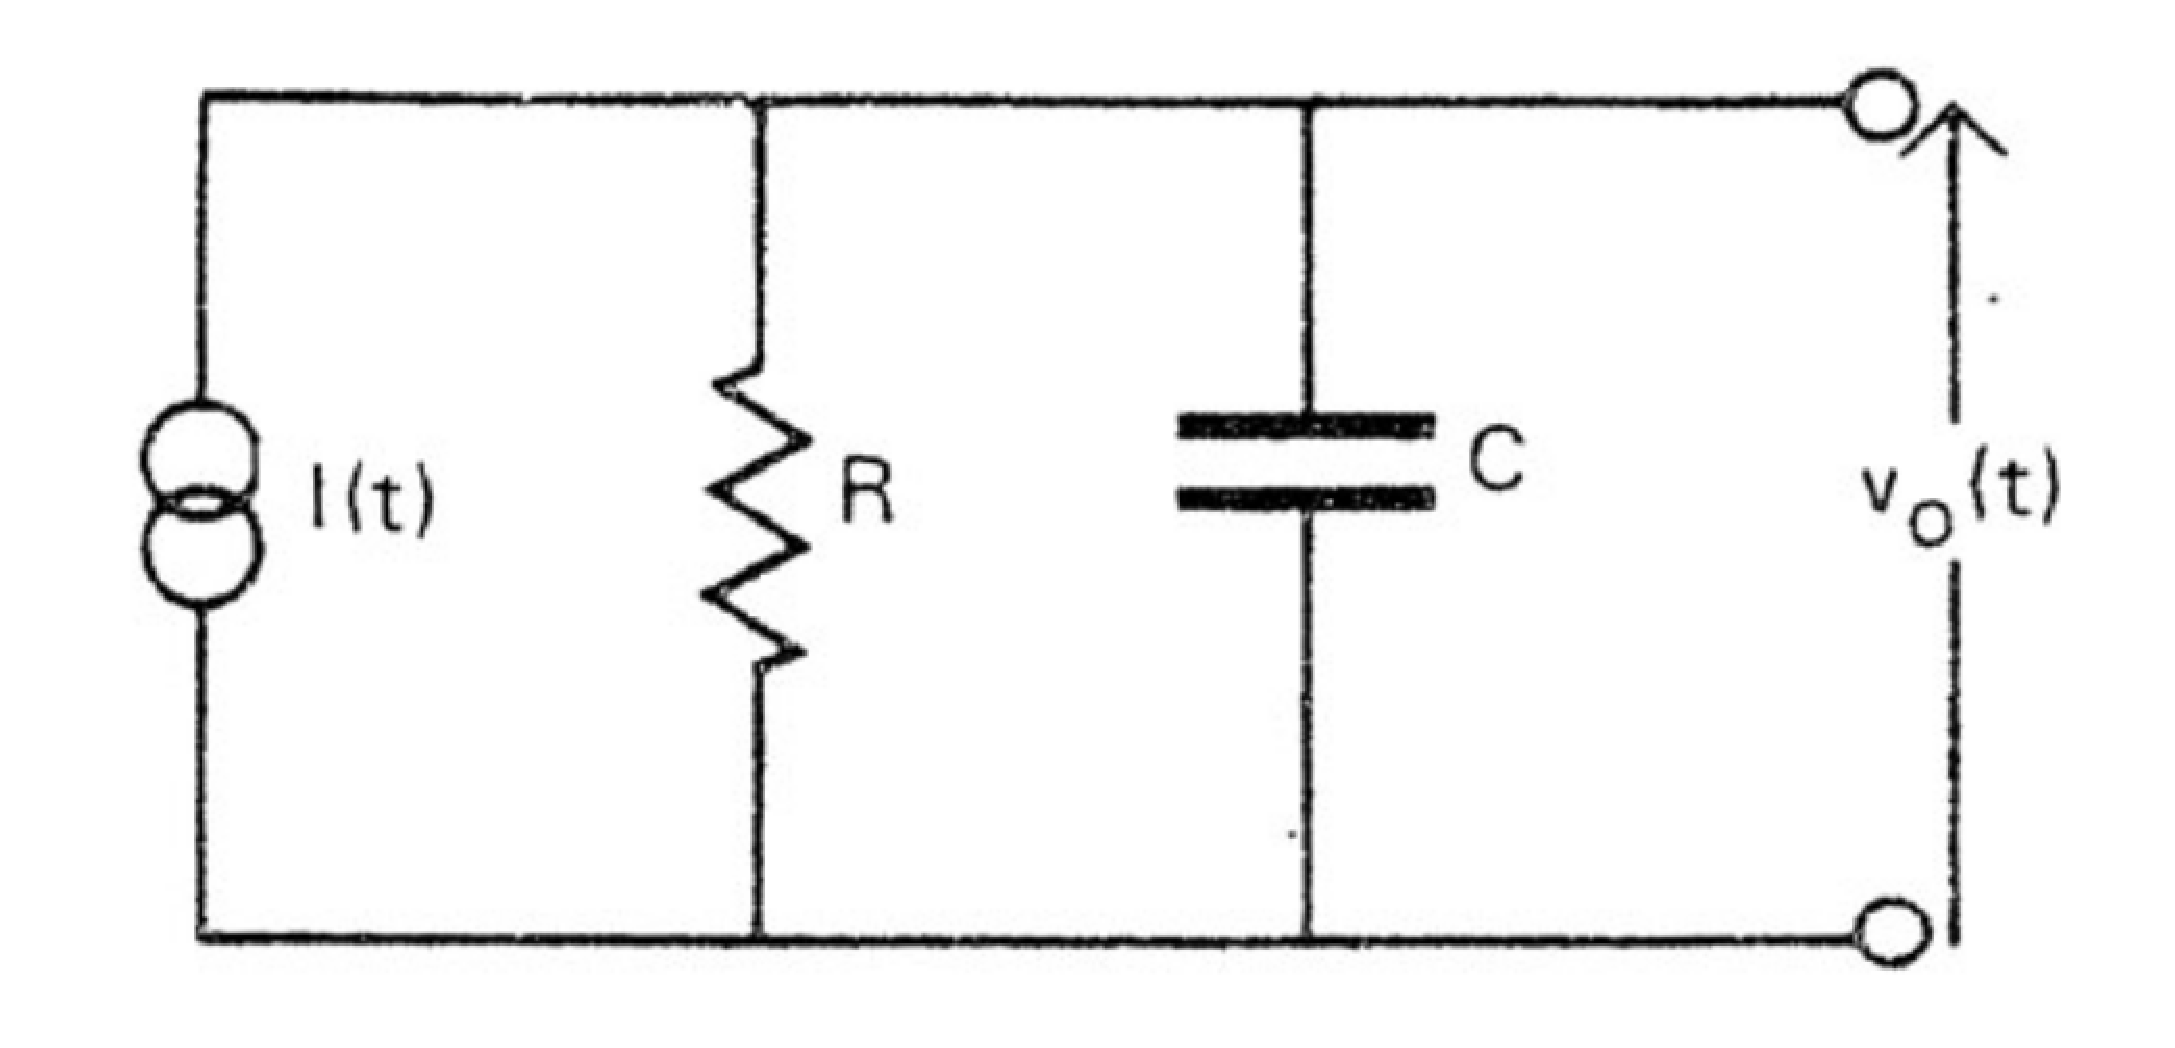
\includegraphics[width=0.6\textwidth]{d1/modelo_PMT}
\end{center}
\end{frame} 

\begin{frame}
\frametitle{Circuito equivalente y señal de salida}
\begin{itemize}
\item La mayoría de las aplicaciones se pueden analizar en términos de una
combinación de R y C
\item Sin pérdida de generalidad, podemos tomar $R = R_0 // R_1$ y $C = C_0 + C_1$
\item Con $R_1$ y $C_1$ las resistencia y capacitancia equivalentes del circuito
de carga
\end{itemize}
\begin{center}
\includegraphics[width=0.7\textwidth]{d1/modelo2_PMT}
\end{center}
\end{frame} 

\begin{frame}
\frametitle{Circuito equivalente y señal de salida}
\begin{block}{}
Consideremos un pulso de luz de salida con decaimiento exponencial en la
intensidad (típico de un centellador, por ejemplo), con una constante
de tiempo $\tau_s$. La corriente de $pe^-$, $I(t)$, viene dada por
$$I(t) = \frac{GNq}{\tau_s}\, e^{(-t/\tau_s)} \quad \text{con}\,N = Nº\,\text{
total de}\,\, pe^- $$

Tenemos entonces una ecuación de la forma 
$$I(t) = \frac{V}{R} + C \frac{dV}{dt}$$

\end{block}
\end{frame} 

\begin{frame}
\frametitle{Circuito equivalente y señal de salida}
\begin{block}{}
Las posibles soluciones ($\tau = RC$)
$$V(t) = - \frac{GNqR}{\tau - \tau_s}\left[e^{(-t/\tau_s)} -
e^{-t/\tau}\right]\qquad \tau \neq \tau_s$$
$$V(t) = - \frac{GNqRt}{\tau_s^2}\,e^{(-t/\tau_s)} \qquad \tau = \tau_s$$
o en función de $C$
$$V(t) = - \frac{GNqt}{(C \tau_s)}\, e^{(-t/\tau_s)} \qquad \tau = \tau_s$$
\end{block}
\end{frame} 

\begin{frame}
\frametitle{Circuito equivalente y señal de salida}
\begin{columns}
\begin{column}{0.5\textwidth}
\begin{center}
\footnotesize{{\color{blue}$R = 50\,\Omega$ y $C$ variable ($\tau_s = 5\,ns$)}}
\includegraphics[width=1.1\textwidth]{d1/ec3_informe}
\end{center}
\end{column}
\begin{column}{0.5\textwidth}
\begin{center}
\footnotesize{{\color{blue}$C = 10\,pF$ y $R$ variable ($\tau_s = 5\,ns$)}}
\includegraphics[width=1.1\textwidth]{d1/ec3R_informe}
\end{center}
\end{column}
\end{columns}
\end{frame}

\begin{frame}
\frametitle{Circuito equivalente y señal de salida}
Podemos sacar algunas conclusiones:
\begin{itemize}
\item La m\'axima amplitud de se\~nal se obtiene para $R \to \infty$. En este
        caso la corriente $I(t)$ simplemente estar\'a cargando el capacitor $C$ y
        la tensi\'on de salida ser\'a

      $$V_o(t) = - \frac{GNq}{C}\, [e^{(-t/\tau_s)} - 1]$$ 

\item Solamente cuando $\tau << \tau_s$ el voltaje de salida ser\'a una 
        reproducci\'on de la corriente $I(t)$ de entrada.
\item El \'area bajo los pulsos es la misma y proporcional a $GNq$.
\item Al considerar el caso $\tau = \tau_s$; cuando $I(t)$ ha deca\'ido dentro
del 1\% de su
      valor inicial, $V(t)$ es todav\'ia $\sim$ 10\% de $V_{max}$. En otras
palabras, el
      pulso de salida tendr\'a un decaimiento largo, que aumenta con $\tau$.
\end{itemize}
\end{frame} 

\begin{frame}
\frametitle{Circuito equivalente y señal de salida}
Podemos sacar algunas conclusiones (cont.):
\begin{itemize}
\item Cuando $R \leq 100\,\Omega$, lo que implica $\tau << \tau_s$, el pulso no
      se integra - esto se denomina {\color{blue}``funcionamiento en modo corriente''} -,
      con el tiempo de subida de los pulsos de corriente y de tensi\'on
      determinado principalmente por la mayor constante de tiempo. Con $\tau
      >> \tau_s$, el pulso de corriente se integra y esta forma de
      funcionamiento se denomina {\color{blue}``modo de tensi\'on''}. Se puede notar c\'omo
      el tiempo de subida (rise time) aumenta a medida que se alcanza el
      ``modo de tensi\'on'' y, en el caso extremo, con $\tau \to \infty$, el 
      tiempo de subida de la tensi\'on es igual al tiempo de decaimiento de la
      entrada.
\item Una constante de tiempo larga es adecuada para bajas tasas de eventos. Si
      la tasa de eventos es $\sim 1/\tau$, ocurre el fen\'omeno de
      acumulamiento (``pulse pile-up'').
\end{itemize}
\end{frame} 

\subsection{Modos de operación}

\begin{frame}
\frametitle{Modos de operación}
\begin{columns}
\begin{column}{0.60\textwidth}
\begin{block}{}
\begin{itemize}
\item Pulsada o digital
\begin{itemize}
\item Photon counting
\item Es la más demandante
\item No funciona bien cuando la intensidad de los fotones incidentes es muy alta y la
electrónica asociada no es lo suficientemente rápida
\item Funciona mejor cuando los fotones incidentes están bien separados temporalmente
\item El número de pulsos es proporcional a la intensidad de la luz incidente  
\item {\color{blue}La altura de los pulsos no es la misma $\rightarrow$ responde al hecho de
que el proceso de multiplicación de $e^-$ es un fenómeno estocástico}
\end{itemize}

%\item Contínua o analógica 
%\begin{itemize}
%\item 
%\end{itemize}
\end{itemize}
\end{block}
\end{column} 
\begin{column}{0.40\textwidth}
\begin{center}
\fbox{\includegraphics[width=0.9\textwidth]{d1/photon_counting_mode}}
\end{center}
\end{column}
\end{columns}
\end{frame} 

\begin{frame}
\frametitle{Modos de operación}
\begin{columns}
\begin{column}{0.60\textwidth}
\begin{block}{}
\begin{itemize}
%\item Pulsada o digital
%\begin{itemize}
%\item Photon counting
%\item Es la más demandante
%\item Requiere electrónica rápida
%\item Funciona mejor cuando los fotones incidentes están bien separados temporalmente
%\end{itemize}

\item Contínua o analógica 
\begin{itemize}
\item Se da cuando la frecuencia de arribo de los pulsos es grande y la
electrónica no puede diferenciar entre pulsos sucesivos 
\item Es una consecuencia del pulse pile-up (acumulamiento)
\item En este modo aparece una corriente media que tiene características
típicas de ruido shot
\end{itemize}
\end{itemize}
\end{block}
\end{column} 
\begin{column}{0.40\textwidth}
\begin{center}
\fbox{\includegraphics[width=0.9\textwidth]{d1/analog_mode}}
\end{center}
\end{column}
\end{columns}
\end{frame} 

\subsection{Redes de polarización}

\begin{frame}
\frametitle{Red de polarización}
\begin{itemize}
\item Requerido para acelerar y enfocar correctamente los electrones
\item Establece los gradientes de potencial requeridos entre etapas (dínodos) 
\item {\color{blue}Mayor potencial en el ánodo}
\item Compuesto por una cadena de $R$ (también puede haber $C$ y transistores)
\item {\color{blue}Su configuración determina el rango dinámico, la linealidad y la ganancia
que tendrá nuestro detector}
\item La fuente de alimentación debe ser estable
\end{itemize}
\begin{center}
\fbox{\includegraphics[width=0.4\textwidth]{d1/tapered_menor_v_last_dyn}}
\end{center}
\end{frame}

\begin{frame}
\frametitle{Red de polarización}
\framesubtitle{Red pasiva}
\only<1>{\begin{center}
\fbox{\includegraphics[width=0.9\textwidth]{d1/tapered_bleeder_circuit}}
\end{center}}
\only<2>{\begin{block}{}
La corriente de la red (\alert{bleeder current}) debe ser mucho mayor que la
corriente del tubo

La variación de ganancia viene dada por 

$$\frac{\Delta G}{G} = \frac{I_{an}}{I_{bl}}\frac{n(1-\delta) +
1}{(1+n)(1-\delta)}$$

$I_{an} \rightarrow$ corriente media de ánodo 

$I_{bl} \rightarrow$ corriente de purga (bleeder) 

$n \rightarrow$ número de etapas

$\delta \rightarrow$ factor de emisión secundario
\end{block}}
\end{frame}

\begin{frame}
\frametitle{Red de polarización}
\framesubtitle{Red activa}
\begin{center}
\fbox{\includegraphics[width=0.9\textwidth]{d1/red_divisora_activa}}
\end{center}
\end{frame}

%\begin{frame}
%\frametitle{La influencia de los capacitores de acople}
%\begin{columns}
%\begin{column}{0.50\textwidth}
%\begin{block}{Electrónica dedicada para Auger}
%\begin{itemize}
%\item Poco flexible 
%\item Información limitada
%\item Número limitado de UBs (\alert{Unified Boards})
%\item Comunicación de datos por puerto serie
%\item	Tiempos de adquisición largos
%\item	Poco volumen de almacenamiento
%\item Sin control línea de base	
%\end{itemize}
%\end{block}
%\end{column} 
%\begin{column}{0.50\textwidth}
%\fbox{\includegraphics[width=\textwidth]{d1/pmt_esquema}}
%\end{column}
%\end{columns}
%\end{frame} 

\subsection{Cálculo de la corriente media de ánodo}

\begin{frame}
\frametitle{Cálculo de la corriente media de ánodo}
\framesubtitle{La corriente de ánodo}
\begin{block}{}
\begin{itemize}
\item $\bar{I}_a$ importa en el diseño de la red de polarización
\item Determina el rango de trabajo donde se asegura cierto grado de
linealidad del circuito
\item Corresponde al producto de la carga por pulso, $Q$, y la
frecuencia de pulsos (que es la misma que la tasa de conteo), $f_p$
$$\bar{I}_a = Q f_p$$
\item Para asegurar variaciones de tensión mínimas, $I_{bl}$ debe ser:
$$I_{bl}/\bar{I}_a \geq 100$$ 
\end{itemize}
\end{block}
\end{frame} 

\begin{frame}
\frametitle{Cálculo de la corriente media de ánodo}
\framesubtitle{Teoría de diseño}
\begin{columns}
\begin{column}{0.5\textwidth}
\begin{itemize}
\item N electrones por segundo generan una $I_k$ 
\item $I_k$ aparece como una corriente de salida, luego de ser amplificada por 3
etapas con ganancia $\delta$ cada una
\end{itemize}
\end{column}
\begin{column}{0.5\textwidth}
\begin{center}
\includegraphics[width=\textwidth]{d1/voltage_div_3_dyn}
\end{center}
\end{column}
\end{columns}
\begin{itemize}
\item Un incremento en $I_k$ causa una caída $\Delta V$ entre $d_3$ y el ánodo
\item Debido a que la $V_{total}$ es constante, $\Delta V$ aparece como un
incremento positivo en las etapas iniciales $d_1$ y $d_2$
\item El efecto se traduce como una variación en la $G_{total}$ del dispositivo
\item \alert{La clave en el diseño del divisor radica en minimizar ese efecto de
realimentación}
\end{itemize}
\end{frame} 

\begin{frame}
\frametitle{Cálculo de la corriente media de ánodo}
\framesubtitle{Teoría de diseño}
Hay dos casos:
\begin{enumerate}
\item Aplicaciones con corriente directa (modo corriente)
\item Aplicaciones pulsadas
\end{enumerate}
\only<1>{\begin{center}
\includegraphics[width=0.5\textwidth]{d1/currents_in_pmt_blanco}
\end{center}}

\only<2>{{\color{blue}Caso 1:}
\begin{itemize}
\item Si $I_k$ es contínua o de variación lenta, entonces, para un tubo de $n$
etapas: $$I_{bl} - I_k \delta^n = I_{bl} - I_a \approx I_{bl}$$
\item Satisfacer la ec. anterior asegura que las tensiones inter-dínodo y por lo
tanto la ganancia permanecerán constantes para $I_a \leq I_{a\, max}$
\end{itemize}}
\only<3>{{\color{blue}Caso 2:}
\begin{itemize}
\item Si $\hat{i}_a$ es una corriente transitoria, resulta necesario mantener
constantes las tensiones inter-dínodo por un tiempo igua a la duración de
$\hat{i}_a$ 
\item Esto puede hacerse colocando $C$ de desacople para entregar la $Q$
requerida por lo pulsos
\item Entonces 
 $$I_{bl} \ll \hat{i}_a \text{, siempre que}\,\, I_{bl} \gg \bar{I}_a$$
\item Donde $\bar{I}_a$ es la corriente media derivada de $\hat{i}_a$ integrada
en un determinado período de tiempo 
\end{itemize}}
\end{frame} 

\subsection{Consideraciones generales}

\begin{frame}
\frametitle{Consideraciones generales}
\framesubtitle{Estabilidad en la ganancia, cambio en la tasa de conteo}
\begin{columns}
\begin{column}{0.60\textwidth}
%\begin{block}{Cambios en la ganancia}
\alert{Cambios en la ganancia}
\begin{itemize}
\item Se puede producir por efecto \alert{fatiga} $\rightarrow$ debido
principalmente a cambios en la cadena de amplificación
\item Se pueden distinguir dos tipos de cambios:
\begin{itemize}
\item \textbf{drift} $\rightarrow$ cambio en el tiempo bajo un nivel constante
de iluminación  
\item \textbf{shift} $\rightarrow$ cambio repentino en la ganancia luego de un
cambio en la corriente (ejemplo: cambio en la ganancia debido a un cambio en la
tasa de conteo)
\end{itemize}
\end{itemize}
%\end{block}
\end{column} 
\begin{column}{0.40\textwidth}
\begin{center}
\includegraphics[width=\textwidth]{d1/shift_and_drift_pmt}
\end{center}
\end{column}
\end{columns}
\end{frame} 

\begin{frame}
\frametitle{Consideraciones generales}
\framesubtitle{Estabilidad en la ganancia, cambio en la tasa de conteo}
\only<1>{Para probar la estabilidad de un PMT se puede usar el siguiente método:

Montar el PMT con un sistema de centelleo y un analizador multicanal. Observar
la distribución de amplitudes de una fuente de $^{137}{Cs}$. En particular notar
la posición del pico de $662\,keV$}

\only<2>{\textbf{Para medir drift} 
\small{\begin{enumerate}
\item Ajustar la distancia de la fuente tal que la tasa de conteo sea $\approx
1000\,s^{-1}$
\item Dejar que el PMT opere con esa tasa por 3 horas
\item Luego una vez cada hora por unas 20 horas, determinar la posición del pico
\end{enumerate}
El drift viene dado por: $$\text{DRIFT} = \frac{\sum_i |\overline{P} -
P_i|}{n\overline{P}}$$

$P_i \rightarrow$ i-ésima medición del pico

$n \rightarrow$ número de mediciones

$\overline{P} \rightarrow$ promedio de $P_i$ sobre todas las $n$ mediciones

\alert{Para un PMT aceptable, el drift no debe superar el 1\%}}}

\only<3>{\textbf{Para medir shift} 
\small{\begin{enumerate}
\item Inmediatamente después de medir el drift, reducir la distancia de la
fuente tal que la tasa de conteo sea $\approx 10000\,s^{-1}$
\item Anotar la medición del pico cada 10 min. para 4 o 5 mediciones
\end{enumerate}
El shift viene dado por: $$\text{SHIFT} = \sum_i \frac{|P_i - P_n|}{mP_n}$$

$P_n \rightarrow$ la última medición hecha para el drift a 1000 cuentas/s

$P_i \rightarrow$ i-ésima medición hecha para shift

$m \rightarrow$ número de mediciones

\alert{Para un PMT aceptable, el shift no debe superar el 1\%}}}
\end{frame}

\begin{frame}
\frametitle{Consideraciones generales}
\framesubtitle{Distribución de amplitudes}
\begin{center}
\fbox{\includegraphics[width=0.5\textwidth]{d1/pulse_height_distribution_pmt}}
\end{center}
Distribución de altura de pulsos de ánodo observados. En un experimento de
conteo de fotones (photon counting) la mejor SNR se obtiene colectando
únicamente los pulsos cuyas amplitudes se encuentran entre la región sombreada
AB.  
\end{frame}

\begin{frame}
\frametitle{Consideraciones generales}
\framesubtitle{Ruido en los PMTs}
\begin{block}{Variadas fuentes}
\begin{itemize}
\item Emisión termoiónica del fotocátodo
\item Emisión termoiónica de los dínodos
\item Emisión por campos altos inter-dínodos
\item Materiales radiactivos en la envoltura del PMT (p. ej. $^{40}K$ en el
vidrio) 
\item $e^-$ golpeando la envoltura del tubo y causando fluorescencia 
\item $e^-$ golpeando los dínodos y causando fluorescencia 
\item Rayos cósmicos
\end{itemize}
\end{block}
\end{frame}

\begin{frame}
\frametitle{Consideraciones generales}
\framesubtitle{Ajuste del voltaje del PMT: Plateau}
\begin{columns}
\begin{column}{0.5\textwidth}
\begin{itemize}
\item El voltaje aplicado al PMT determina su ganancia y entonces la altura de
los pulsos de salida
\item A veces es necesario ajustar la tensión aplicada teniendo en cuenta
efectos de saturación o de corrientes excesivas
\end{itemize}
\end{column}
\begin{column}{0.5\textwidth}
\begin{center}
\includegraphics[width=0.5\textwidth]{d1/plateau}
\end{center}
\end{column}
\end{columns}
\end{frame}

\begin{frame}
\frametitle{Consideraciones generales}
\framesubtitle{Ajuste del voltaje del PMT: Plateau}
\begin{columns}
\begin{column}{0.5\textwidth}
\begin{itemize}
\item Es un procedimiento usado para encontrar el voltaje de trabajo adecuado en
photon counting 
\item Representa la zona en la que el conteo es menos sensible a cambios de
voltaje 
\item La segunda ``subida'' marca el efecto de regeneración (afterpulsos,
descargas, etc)
\end{itemize}
\end{column}
\begin{column}{0.5\textwidth}
\begin{center}
\includegraphics[width=0.9\textwidth]{d1/plateau2}
\end{center}
\end{column}
\end{columns}
\end{frame}

\begin{frame}
\frametitle{Consideraciones generales}
\framesubtitle{Señal del último dínodo}
\begin{block}{Se elige la señal del último dínodo debido a que:}
\begin{itemize}
\item La señal del dínodo se produce simultáneamente con la
salida del ánodo, de modo que se puede utilizar como
señal de temporización de eventos.
\item Puede utilizarse en conjunto con la señal del ánodo para
extender el rango dinámico de la medición.
\item La señal tomada del último dínodo tiene una amplitud
comparable con la del ánodo y tiene una mayor relación
señal/ruido que los otros dínodos.
\item La señal del último dínodo tiene polaridad opuesta a la
del ánodo.
\end{itemize}
\end{block}
\end{frame}

%------------------------------------------------------------------------------
\section{Los fotomultiplicadores de silicio (SiPM)}
%------------------------------------------------------------------------------

\begin{frame}
\begin{center}
\Huge{\color{blue}{Los SiPM (o MPPC)}} \\
\begin{center}
\fbox{\includegraphics[width=0.8\textwidth]{d1/sipm_portada}}
\end{center}
\end{center}
\end{frame}

\begin{frame}
\frametitle{Introducción}
\begin{block}{}
\begin{itemize}
\item Los MPPC son un nuevo tipo de dispositivos para el conteo de fotones
compuestos por múltiples píxels de APD (avalanche
photodiode) funcionando en modo Geiger
\item Son esencialmente dispositivos opto-semiconductores con excelentes
capacidades de conteo de fotones
\item Tienen ventajas respecto a otros dispositivos, tal como el bajo voltaje de
operación y la insensibilidad a los campos magnéticos 
\end{itemize}
\end{block}
\begin{center}
\includegraphics[width=0.4\textwidth]{d1/sipm_varios}
\end{center}
\end{frame}

\begin{frame}
\frametitle{Introducción}
\begin{block}{Características sobresalientes}
\begin{itemize}
\item Excelente capacidad de conteo de fotones (excelente eficiencia de
detección vs. número de fotones incidentes)
\item Tamaño pequeño
\item Operación a temperaturas de laboratorio
\item Baja tensión de trabajo (debajo de 80 V)
\item Alta ganancia: $10^5$ a $10^6$
\item Excelente resolución temporal
\item Insensible a campos magnéticos
\item Circuitería de lectura simple
\end{itemize}
\end{block}
\end{frame}

\begin{frame}
\frametitle{Principio de operación}
\framesubtitle{Modo Geiger}
\begin{center}
\includegraphics[width=0.8\textwidth]{d1/curva_sipm}
\end{center}
\end{frame}

\begin{frame}
\frametitle{Principio de operación}
\framesubtitle{Estructura}
\begin{center}
\fbox{\includegraphics[width=0.9\textwidth]{d1/sipm_operation}}
\end{center}
\end{frame}

\subsection{EL circuito equivalente del SiPM}

\begin{frame}
\frametitle{Principio de operación}
\framesubtitle{Circuito equivalente}
\begin{center}
\includegraphics[width=0.5\textwidth]{d1/sipm_equiv_circ}
\end{center}

$R_q \rightarrow$ R de enfriamiento (quenching)

$C_q \rightarrow$ C parásita

$C_d\,\,\text{y}\,\,C_g \rightarrow$ C asociadas a la microcelda y a las
conexiones ($30-50\,\text{fF}$)
\end{frame}

\begin{frame}
\frametitle{Principio de operación}
\framesubtitle{Lectura de la señal de salida}
\includegraphics[width=0.8\textwidth]{d1/readout_sipm}
\end{frame}

\begin{frame}
\frametitle{Principio de operación}
\framesubtitle{Lectura de la señal de salida}
Se pueden usar dos métodos para estimar el número de fotones detectados por el SiPM

\only<2>{
\alert{Observando los pulsos de salida (amplitud)}
\begin{center}
\includegraphics[width=0.6\textwidth]{d1/pulso_sipm}
\end{center}}

\only<3>{
\alert{Midiendo la carga de salida}
\begin{center}
\includegraphics[width=0.4\textwidth]{d1/sipm_spectrum}
\end{center}}
\end{frame}

%%------------------------------------------------------------------------------
%\section{Señales pulsadas en electrónica nuclear}
%%------------------------------------------------------------------------------
%
%\subsection{Terminología}
%\subsection{Señales analógicas y digitales}
%\subsection{Señales rápidas y señales lentas}
%\subsection{El dominio de la frecuencia. Ancho de banda}
%
%%------------------------------------------------------------------------------
%\section{Transmisión de señales}
%%------------------------------------------------------------------------------
%
%\subsection{Cables coaxiales}
%\subsubsection{Impedancia característica}
%\subsubsection{Reflexiones}
%\subsubsection{Terminación de cables: adaptación de impedancias}
%\subsubsection{Pérdidas en cables coaxiales. Distorsión de pulsos}
%\subsubsection{Respuesta del cable. Distorsión de pulsos}

\begin{frame}
\begin{center}
%\huge{¡Muchas Gracias!}
\includegraphics[height=0.6\textheight,width=0.65\textwidth]{gracias}
\end{center}
\end{frame}

\begin{frame}
\begin{center}
\huge{¿Preguntas?}\\
\vspace{5mm}
\includegraphics[height=0.4\textheight,width=0.4\textwidth]{preguntas}
\end{center}
\end{frame}


\end{document}
